\chapter{Implementation}
\label{ch:Implementation}
This chapter delves into the detailed implementation of the methodologies outlined in \autoref{ch:Methodology}, focusing on the specific processes, experiments, and analyses conducted. It includes the practical steps taken to prepare data, apply distortions, extract features, and train the regression model to assess image quality in teledermatology.

\section{Image Selection and Labeling Process}
\label{sec:ImgSelectLabel}
This section describes the initial stages of the implementation, focusing on the selection and preparation of the image datasets used in the study. \par
\vspace{\baselineskip}
\noindent

\subsection{Image Filtering and Selection}
\label{sub:ImgFilterSelect}
The first step in preparing the images involves carefully choosing high-quality pictures from the SCIN dataset, which mainly includes pictures of early-stage dermatological conditions. This selection is done manually as it ensures that each image is clear and useful for clinical use. The primary focus during selection is for images that are well-framed and free of any distortions that might affect their usefulness in diagnosis.\par
\vspace{\baselineskip}
\noindent
Each selected image is checked to make sure it doesn't have any blurring that might hide important details of the skin condition, as clear images are crucial for accurate diagnosis. Additionally, it's important that the images are properly lit and show true contrast, this means they shouldn't be too bright or too dark. Proper lighting and contrast help in accurately showing the skin's condition. Lastly, the images must represent realistic skin tones and colors. Accurate color representation is critical because wrong colors can lead to incorrect diagnoses. This careful selection process of images ensures that the baseline images used for further distortion and analysis are of good quality, providing a solid foundation for the subsequent experimental stages. \par


\subsection{Labeling of the Test Set}
\label{sub:LabelingTestSet}
The labeling process involves manually scoring approximately 50 high-quality images and 200 images with various distortions. These images are evaluated based on seven key quality criteria crucial for teledermatology: lighting, focus, orientation, color calibration, background, resolution, and field of view. Each image is scored on a scale from 0 to 1 for each criterion, where 0 indicates no distortion and 1 indicates extreme distortion. \par
\vspace{\baselineskip}
\noindent
This manual labeling is facilitated through a custom Python script, which displays each image and prompts the user to enter scores for each distortion criterion. The scores are collected in a structured format and stored in a JSON file for subsequent analysis. This structured and meticulous approach ensures that each image is evaluated consistently and comprehensively.\par
\noindent
\subsubsection{Visualization of Label Distribution}
\label{subsub:LabelDist}
To understand the distribution of labels and how frequently distortions occur across different criteria, histograms are generated. These histograms are particularly useful for visualizing the prevalence and severity of distortions in the dataset. Two histograms are plotted for each criterion:\par
\vspace{\baselineskip}
\noindent
The first histogram shows the distribution of images scored as '0' for a specific criterion, representing images where no distortion is observed. \par
\noindent
The second histogram displays the distribution for images where a distortion is present (scores >0), showing the varying levels of distortion severity.\par
\vspace{\baselineskip}
\noindent
These histograms provide valuable insights into the commonality and impact of each type of distortion, aiding in the analysis of how distortions affect overall image quality. They also highlight the criteria that may require more focused attention during the model training and validation process. \par
\todo{Histogram: "Distribution of images scored as 0 for the focus criterion, indicating no distortion." or "Distribution of scores for the focus criterion where distortion is present, illustrating the range and frequency of severity."}

\section{Distortion Pipeline}
\label{sec:DistPipeline}
The distortion pipeline is central to simulating realistic image quality issues. Each quality criterion has multiple types of distortions, each having five ranges of intensity, increasing in severity. All distortion types begin at zero, indicating no distortion applied, and progress to higher values that represent increasing levels of the specified distortion. Visual representations of the types of degradations at different ranges for each quality criterion is provided in the \autoref{ch:Supplementary}.  \par
\vspace{\baselineskip}
\noindent
This section describes each distortion type and its impact on image quality, highlighting the adaptability of the pipeline in generating training images that reflect a range of realistic conditions. \par

\subsection{Distortion Types}
\label{sub:DistTypes}
Here, each distortion type is briefly described, highlighting how they simulate different aspects of image degradation: \par
\begin{enumerate}
    \item Lighting:
        \begin{itemize}
            \item \textit{Brighten}: applies a sequence of color space transformations, curve adjustments, and blending operations to enhance the brightness of an input image, resulting in an output image with increased visual intensity;
            \item \textit{Darken}: similar to brighten operation, but it leads to a decreased visual intensity;
        \end{itemize}
    \item Focus:
        \begin{itemize}
            \item \textit{Gaussian blur}: filters every pixel of the image with a simple Gaussian kernel.
            \item \textit{Lens blur}: filters every pixel of the image with a circular kernel;
            \item \textit{Motion blur}: filters every pixel of the image with a linear motion blur kernel to simulate the effect of a moving camera or a moving object in the scene. Consequently, the image appears blurred in the direction of the motion;
        \end{itemize}
    \item Orientation:
        \begin{itemize}
            \item \textit{Top perspective}: temp;
            \item \textit{Bottom perspective}: temp;
            \item \textit{Left perspective}: temp;
            \item \textit{Right perspective}: temp;
        \end{itemize}
    \item Color calibration:
        \begin{itemize}
            \item \textit{Color saturation 1}: converts the image to the HSV-color space and then multiplies the saturation channel by a factor;
            \item \textit{Color saturation 2}: converts the image to the LAB-color space, then multiply each color channel by a factor;
        \end{itemize}
    \item Background:
        \begin{itemize}
            \item \textit{temp}: temp;
        \end{itemize}
    \item Resolution:
        \begin{itemize}
            \item \textit{temp}: temp;
        \end{itemize}
    \item Field of view:
        \begin{itemize}
            \item \textit{temp}: temp;
        \end{itemize}
\end{enumerate}

\section{Distortion Implementation Process}
\label{sec:DistProcess}

\begin{figure}[ht]
    \centering
    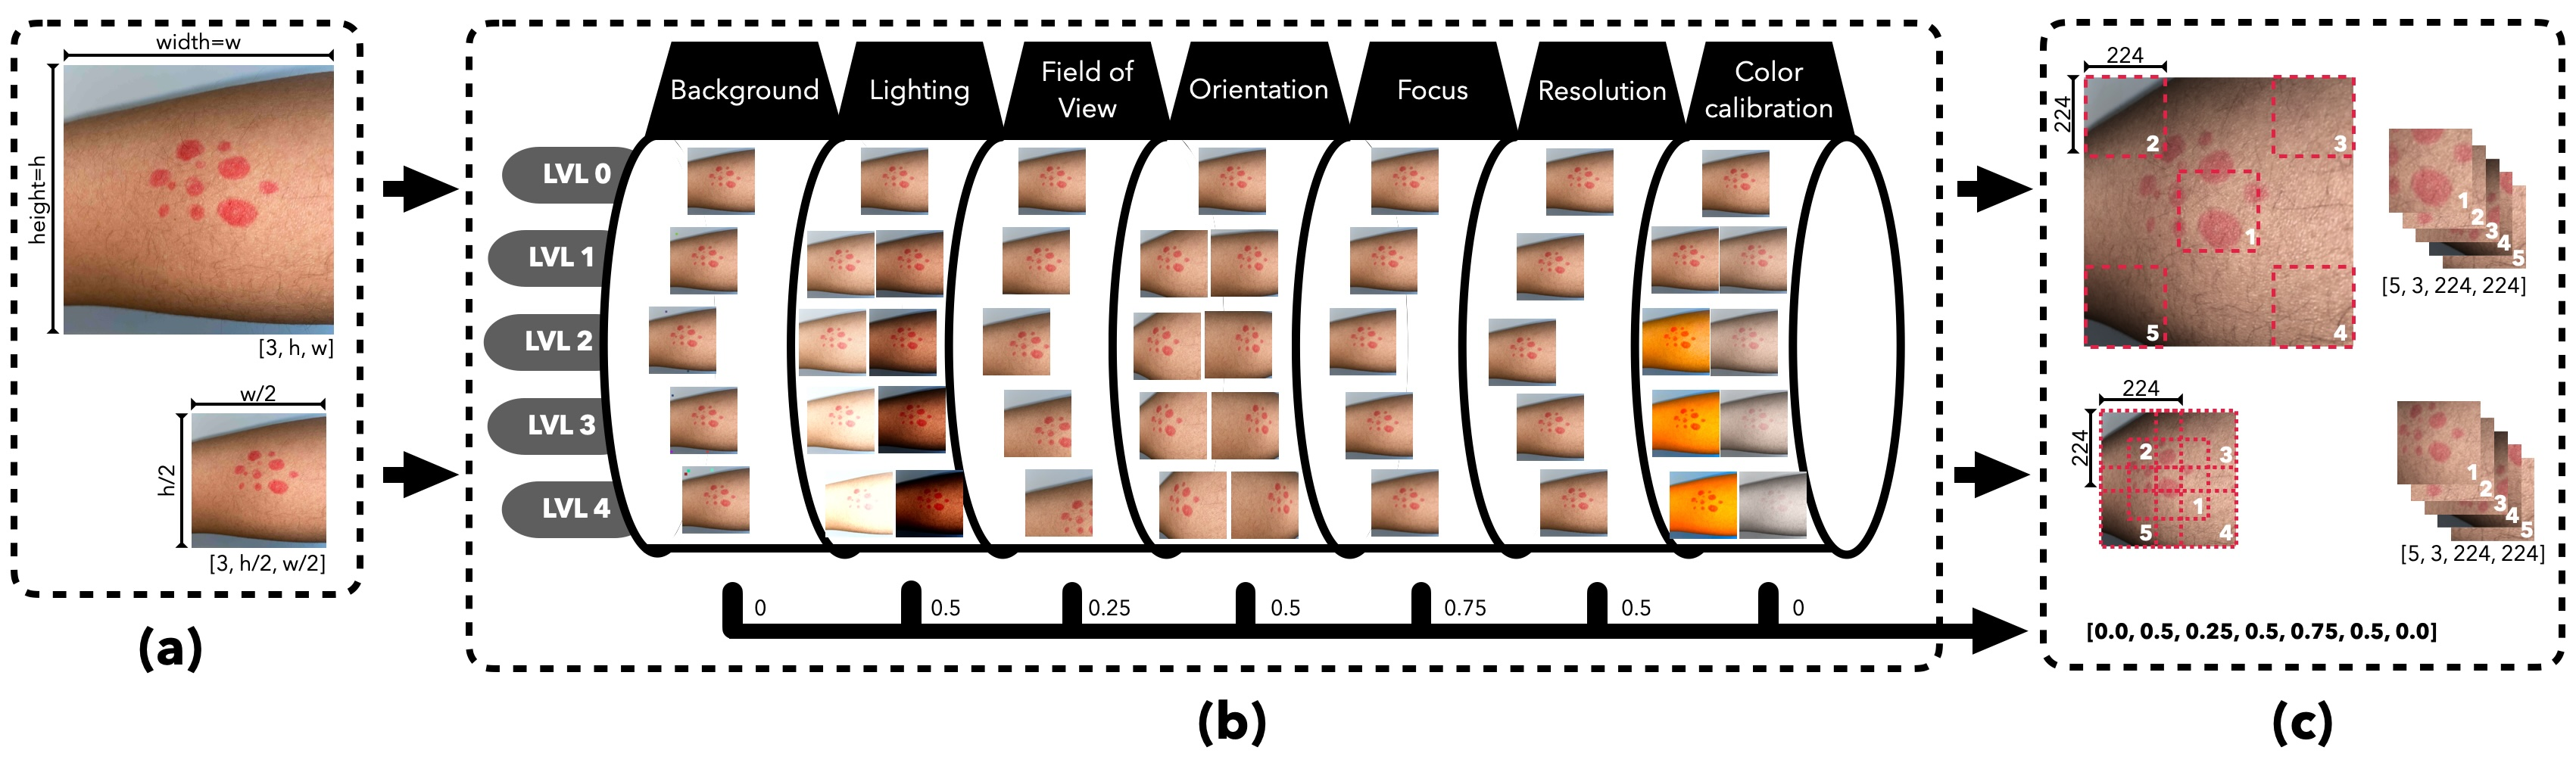
\includegraphics[keepaspectratio,width=15cm]{img/Distortion_pipeline.jpg}
    \caption{Distortion pipeline for generating training images with varying levels of distortion.}
    \label{fig:DistPipeline}
\end{figure}

The good quality images selected from the SCIN \autocite{SCIN} dataset are processed, where each image is first resized to a target resolution of 512 pixels while maintaining the aspect ratio. This resizing is crucial to standardize the input size and improve the consistency of feature extraction across different images. For each image, a downsampled version is created. The downsampled image serves as a means to generate hard negative examples, enhancing the learning process. \par
\vspace{\baselineskip}
\noindent
The images then undergo a series of distortions through a defined pipeline, as mentioned in \autoref{sec:DistPipeline}, which applies a sequence of distortion functions. These functions are chosen based on a Gaussian distribution with a mean of 0 and a standard deviation of 2.5, ensuring a probabilistic variation and to add a realistic randomness in the severity of applied distortions. The distortion values are mapped to a uniform scale from 0 to 1, representing the intensity of the distortion from none to extreme. This mapping is crucial for training the model to recognize and quantify these distortions accurately. \par
\begin{table}[h]
    \centering
    \begin{tabularx}{\textwidth}{|X|X|X|X|X|}
        \hline
        \textbf{0} & \textbf{0.25} & \textbf{0.5} & \textbf{0.75} & \textbf{1} \\ \hline
        No distortion applied & Slight distortion & Moderate distortion & Significant distortion & Extreme distortion \\ \hline
    \end{tabularx}
    \caption{Mapping of numerical values to levels of distortion.}
    \label{tab:a}
\end{table}

\noindent
After the distortions are applied, both the original and downsampled images are processed to extract smaller crops from significant areas such as the center and the four corners. This step is vital as it ensures that the model learns from various perspectives within the same image, enhancing the robustness of the learned features. The crops are then stacked to form a batch of images ready for feature extraction. But first, the images are normalized using standard values (mean=[0.485, 0.456, 0.406], std=[0.229, 0.224, 0.225]) \todo{Using the mean and std of Imagenet is a common practice. They are calculated based on millions of images. If you want to train from scratch on your own dataset, you can calculate the new mean and std. Otherwise, using the Imagenet pretrianed model with its own mean and std is recommended.} to match the input requirements of the neural network used in SimCLR. This normalization helps in stabilizing the training process by scaling the input features to a common range. \par
\vspace{\baselineskip}
\noindent
The prepared images are then passed through the SimCLR network to extract features. The network maximizes the similarity of embeddings from images degraded in a similar manner while maximizing the dissimilarity with embeddings from different images or from downsampled versions, which serve as hard negative examples. \par

\begin{figure}[ht]
    \centering
    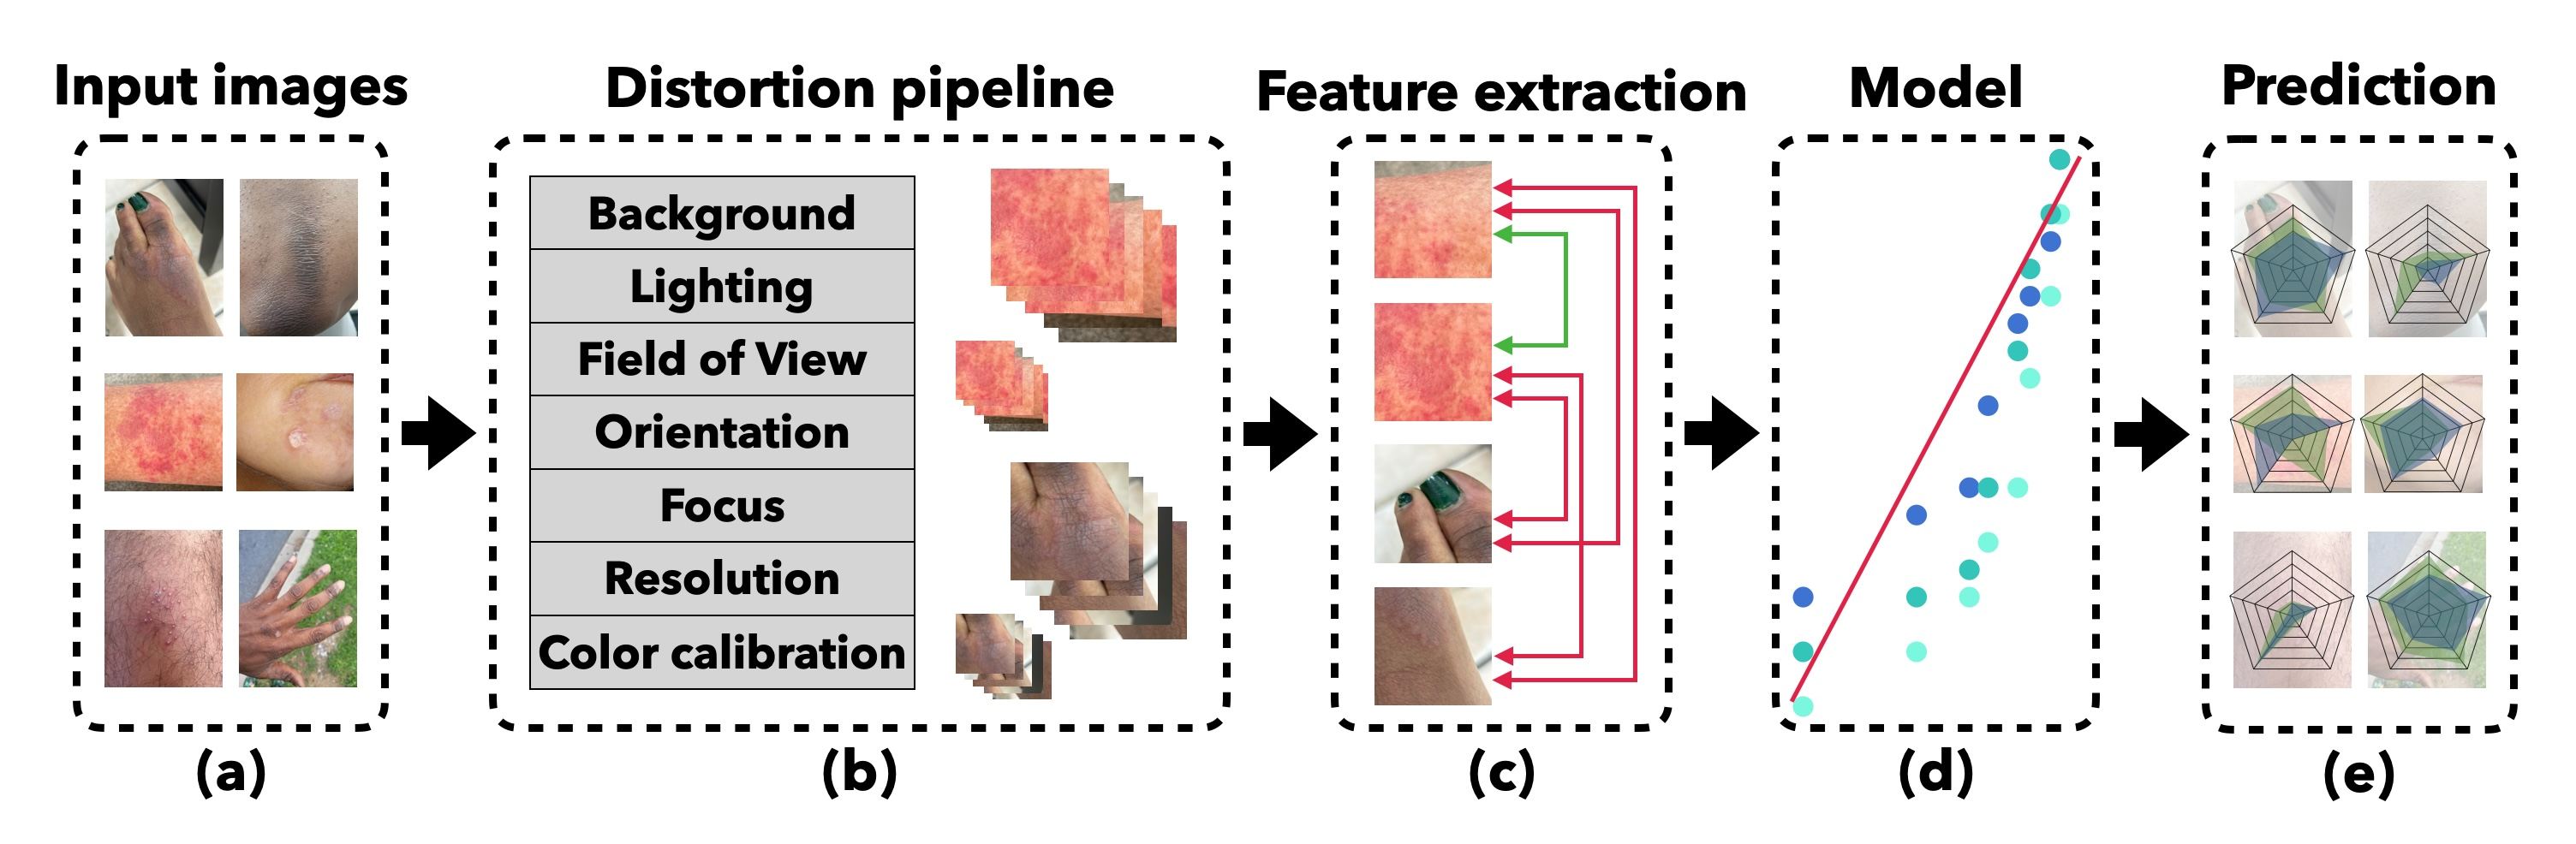
\includegraphics[keepaspectratio,width=15cm]{img/Architecture.jpg}
    \caption{Architecture.}
    \label{fig:Architecture}
\end{figure}

\section{Feature Extraction with SimCLR}
\label{sec:FeatureExtraction}
Once the crops from the distorted and downsampled images have been generated, they are processed through the SimCLR framework implemented within the ARNIQA system to extract meaningful features. SimCLR, a pivotal component of ARNIQA, operates based on a self-supervised contrastive learning approach. This framework is adept at maximizing the similarity of features between images that have been distorted in a similar manner, regardless of their initial content. \par


The implementation of the SimCLR framework from ARNIQA forms a pivotal part of the feature extraction process for this project. SimCLR stands out due to its robust self-supervised learning capabilities, particularly suited for handling the complex distortions applied to the images in this study.

Overview of SimCLR in ARNIQA:

SimCLR operates by maximizing the similarity between embeddings of differently cropped images from the same source but subjected to identical distortions, while also minimizing their similarity to embeddings from differently distorted crops. This methodology effectively trains the model to recognize and quantify similar degradation patterns across diverse image content, leveraging a contrastive loss function that is critical for learning detailed distortion characteristics.

Training Strategy with SimCLR:

The training strategy involves processing pairs of images through a series of steps:

Image Pair Selection: Two pristine images are selected randomly from the dataset.
Distortion Application: Each image is cropped and subjected to the same distortion, based on predefined distortion compositions.
Embedding Comparison: The embeddings of the distorted image crops are compared to ensure that similar distortions produce similar embeddings.
This process is visualized in Figure 3 from the ARNIQA paper, which illustrates how the embeddings of similarly degraded image crops are aligned, while those of differently degraded crops serve as hard negative examples. This setup is crucial for training the model to discriminate subtle differences in degradation, enhancing its sensitivity to variations in image quality.

Hard Negative Examples:

To enhance the model’s ability to discern subtle degradation differences, images are also downscaled before cropping and distorting, creating hard negative examples. These examples are crucial for training because they share similar content but differ in distortion due to the downsampling process, challenging the model to fine-tune its discrimination capabilities.

Reproducibility and Practical Implementation:

The availability of code and weights for the SimCLR implementation in ARNIQA ensures that this methodology is not only reproducible but also accessible for future research. This open access to resources supports ongoing improvements and adaptations in the field, fostering further developments in image quality assessment for teledermatology.

Benefits of SimCLR in Image Quality Assessment:

Utilizing SimCLR provides significant advantages:

Unlabeled Data Usage: It can effectively learn from unlabeled data, which is particularly beneficial in scenarios where high-quality labeled datasets are scarce.
Robust Feature Extraction: By learning to identify and differentiate between various image distortions, SimCLR helps in building a robust model capable of accurate image quality assessment.
Enhanced Learning from Distortions: The framework’s focus on maximizing similarity for similarly distorted images and maximizing dissimilarity for differently distorted images (even when content is similar) enables the model to learn a comprehensive distortion manifold.
These capabilities make SimCLR an ideal choice for this project, addressing the challenges of assessing image quality in teledermatology where diverse and subtle image distortions can significantly impact diagnostic accuracy. The implementation details and insights gained from using SimCLR are foundational for the subsequent stages of model training and validation discussed in the following sections. \par
\vspace{\baselineskip}
\noindent

\subsection{Framework Details}
\label{sub:FrameworkDetails}


\section{Regression Model Training and Validation}
\label{sec:ModelTrainVal}
text \par
\vspace{\baselineskip}
\noindent

\subsection{Model Selection and Training}
\label{sub:ModelTraining}

\subsection{Performance Metrics}
\label{sub:PerfMetrics}


\section{Model Testing}
\label{sec:ModelTesting}
The final model is tested against the labeled test set to evaluate its performance in real-world scenarios. Plots illustrating the model’s performance across various quality criteria will be shown, highlighting areas where the model performs well or where there is significant variance, indicating uncertainty in quality assessment. \par
\vspace{\baselineskip}
\noindent

\subsection{Testing with Labeled Test Set}
\label{sub:TestLabeledSet}